\chapter{Time-Resolved Emittance Measurements}

\section{Introduction}

\subsection{What is Emittance}
 

\subsection{What Emittance is useful for}

\section{Theory}

A given ensemble of particles can be described by its density in six-dimensional phase space, $(x, p_x, y, p_x, z, p_z)$ where $(x, y, z)$ are the positions and $(p_x, p_y, p_z)$ are the momenta of each particle.
The extent of the beam in phase space is called the \emph{emittance} of the beam.
Each cartesian direction is usually examined separately, $(x, p_x)$, $(y, p_y)$ and $(z, p_z)$ where $z$ is the optic axis of the beam.

Typically the gradients of trajectories in $x$-$z$ and $y$-$z$ are measured rather than the momenta.
These gradients are referred to as the divergence and are defined as $x^\prime \equiv \frac{dx}{dz} = \frac{v_x}{v_z}$.
The space of $(x, x^\prime)$ is referred to as trace-space. The \emph{emittance} can be defined as
\begin{equation}
\epsilon^x \equiv \frac{A^x}{\pi}
\end{equation}
where $A^x$ is the area occupied by the beam in trace space.

The density, $\rho$, of a beam of $N$ particles in trace space can usually be described by a Gaussian:
\begin{equation}\label{trace_space_density}
\rho(x, x^\prime) = N exp\left[ \frac{-(\sigma_{22}x^2-2\sigma_{12}xx^\prime+\sigma_{11}x^{\prime2}}{2|\sigma|} \right]
\end{equation}
where $|\sigma|$ is the determinant of the symmetric beam matrix,
\begin{equation}
\sigma = \begin{pmatrix} \sigma_{11} & \sigma_{12} \\ \sigma_{21} & \sigma_{22} \end{pmatrix}
\end{equation}
$\sigma_{11}$ is the standard deviation of $x$, $\sigma_{22}$ the standard deviation of $x^\prime$ and $\sigma_{12}=\sigma_{21}$ indicates the coupling between $x$ and $x^\prime$. The \emph{emittance} can also be defined as
\begin{equation}\label{eq:emittancewithdeterminant}
\epsilon^x \equiv \sqrt{|\sigma|} = \sqrt{\sigma_{11}\sigma_{22}-\sigma_{12}^2}
\end{equation}

The \emph{\gls{rms} emittance} of the ensemble can be defined as
\begin{equation}\label{emittance}
\epsilon \equiv \sqrt{\langle x^2\rangle \langle x^{\prime 2}\rangle - \langle x x^\prime\rangle^2}.
\end{equation}

\section{Measurement}

Directly calculating the emittance of an ensemble with Eq. \ref{emittance} requires full knowledge of the position and momenta of the particles which is difficult as beam monitors tend to only measure the transverse positions of particles.
There are a number of methods to practically calculate the emittance of a particle beam, namely pepperpots, the multiple profile method methods and the quadrupole method.

\subsection{Pepperpots}

\subsection{Multi-profile Method}

If a beam can be described by $\sigma^0$ at $z_0$ and by $\sigma^1$ at $z_1$ then the transformation matrix, $\mathbf{R}_{12}$ from $z_0$ to $z_1$ is
\begin{equation}
\mathbf{R} = \begin{pmatrix} R_{11} & R_{12} \\ R_{21} & R_{22} \end{pmatrix}
\end{equation}
and
\begin{equation}
\sigma^1 = \mathbf{R}\sigma^0\mathbf{R}^T
\end{equation}
where $\mathbf{R}^T$ is the transpose of $\mathbf{R}$.
The combined transfer matrix for a series of $z$ positions is simply the product of the individual transfer matrices.

We can write:
\begin{equation}\label{multiprofileequation}
\sigma_{11}^1 = R_{11}^2\sigma_{11}^0 + 2R_{11}R_{12}\sigma_{12}^0 + R_{12}^2\sigma_{22}^0
\end{equation}

Typical detectors are only able to measure the standard deviation of $x$, $\sigma_{11}$.
With at least three measurements and known transfer matrices the other elements of $\sigma$ can be determined.
With more than three measurements uncertainty can be reduced.

The transfer matrix for simple propagation over a distance $L$ is
\begin{equation}
\mathbf{R}_L = \begin{pmatrix}1 & L \\ 0 & 1\end{pmatrix}
\end{equation}
and then Eq.~\ref{multiprofileequation} becomes
\begin{equation}
\sigma_{11}^1 = \sigma_{11}^0 + 2L \sigma_{12}^0 + L_1^2\sigma_{22}^0.
\end{equation}

\begin{figure}
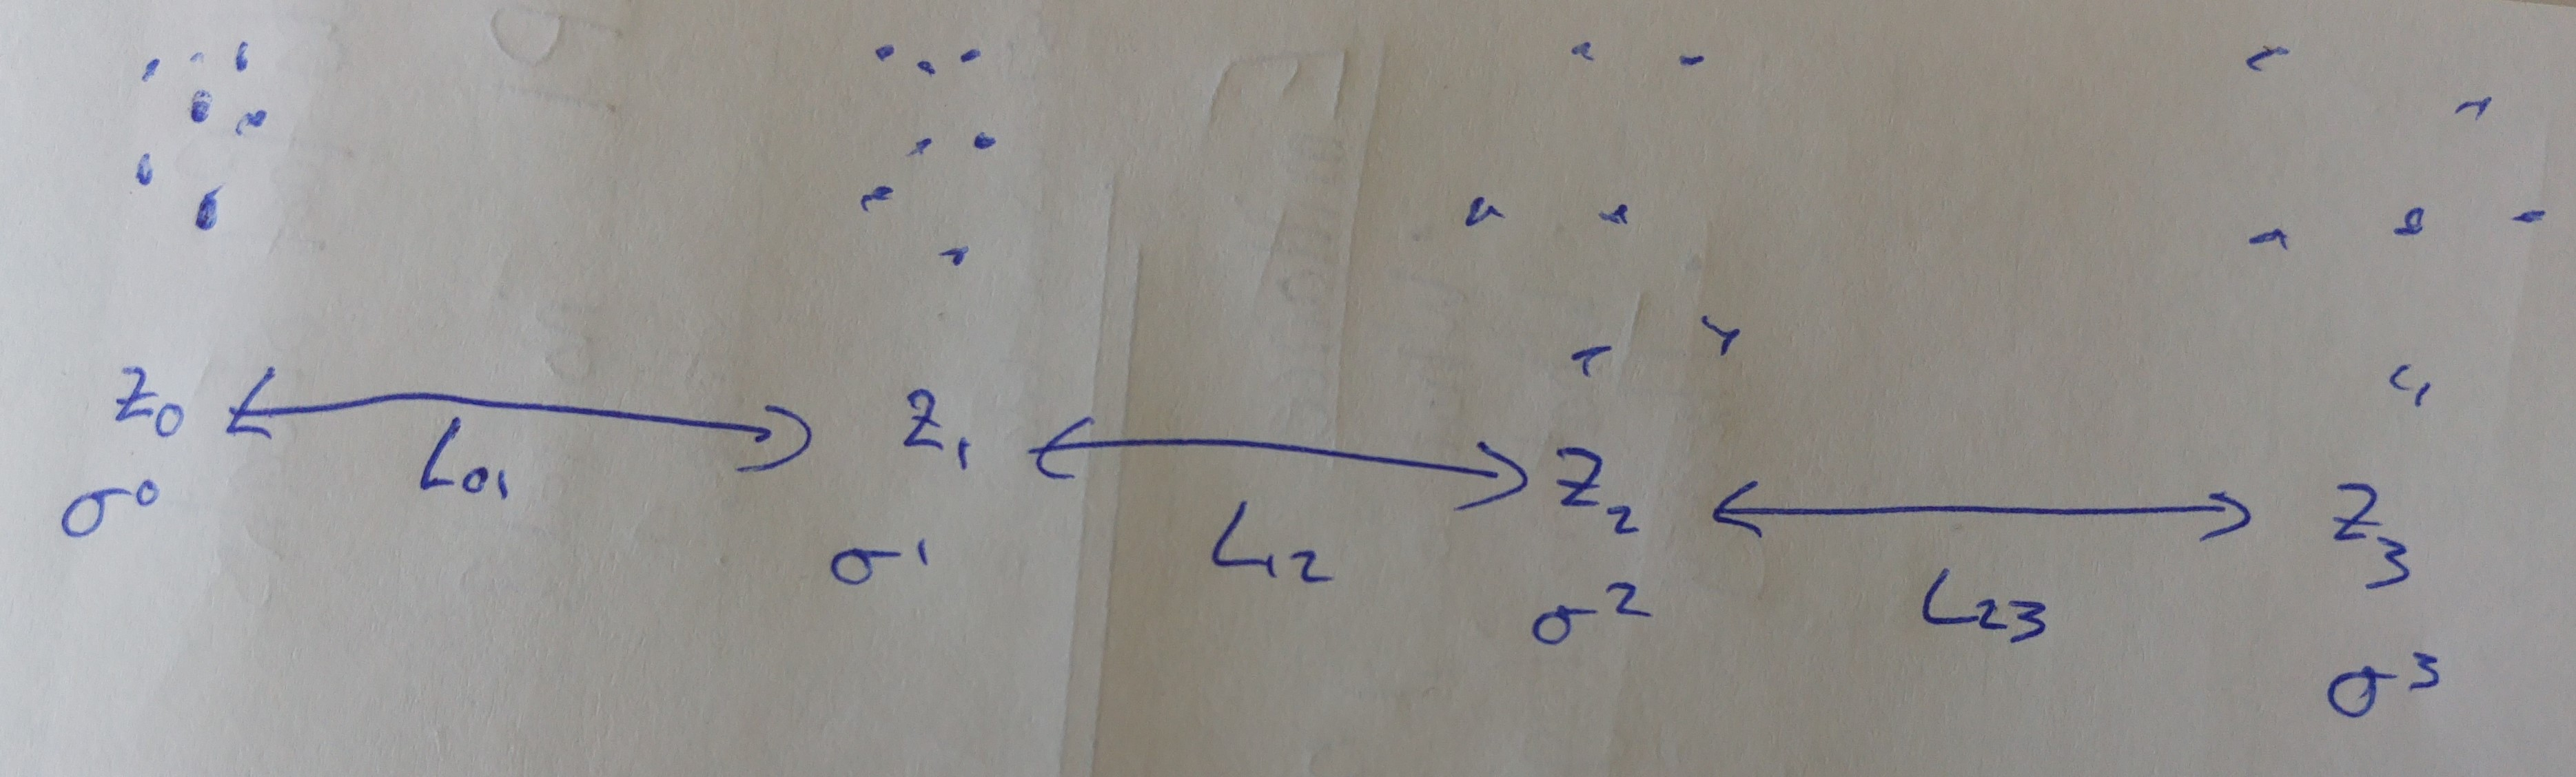
\includegraphics[width=\linewidth]{part2/Figs/multiprofileexample.jpg}
\caption{An example of a multi-profile emittance measurement. {\color{red}Add R matrices. Perhaps express $L_{01}$, $L_{02}$ and $L_{03}$ instead? Appropraitely update Eq.~\ref{eq:multiprofilesolution}}}
\label{figure:multiprofileexample}
\end{figure}

With an initial beam, $\sigma_0$, measured at $z_1, z_2$ and $z_3$ as shown in Fig.~\ref{figure:multiprofileexample} then $\sigma_{11}^1$, $\sigma_{11}^2$, and $\sigma_{11}^3$ are know and we can write 
\begin{align}
\sigma_{11}^1 &= \sigma_{11}^0 +2L_{01}\sigma_{12}^0 + L_{01}^2\sigma_{22}^0 \notag\\
\sigma_{11}^2&= \sigma_{11}^0+2(L_{01}+L_{12})\sigma_{12}^0 + (L_{01}+L_{12})^2\sigma_{22}^0 \notag\\
\sigma_{11}^3&= \sigma_{11}^0+2(L_{01}+L_{12}+L_{23})\sigma_{12}^0 + (L_{01}+L_{12}+L_{23})^2\sigma_{22}^0 \label{eq:multiprofilesolution}
\end{align}

Which can easily be solved for $\sigma_0$ thus allowing the calculation of the emittance with Eq.~\ref{eq:emittancewithdeterminant}.

\subsection{Quadrupole Method}

The quadrupole method is similar to the multi-profile method but requires only a single location to measure the beam width and a well characterised variable lens such as a quadrupole lens.
A quadrupole lens with a magnetic field gradient of $G$ has the transfer matrix in the focusing plane of
\begin{equation}
\mathbf{R}_f = \begin{pmatrix} \cos kl & (1/k)\sin kl\\
-k\sin kl & cos kl\end{pmatrix},
\end{equation}
where $l$ is the effective length of the quadrupole, $k^2=G/B\rho$ is the quadrupole strength and $B\rho$ is the magnetic rigidity of the particles in the assumed central trajectory.
The matrix in the defocusing palne is
\begin{equation}
\mathbf{R}_d = \begin{pmatrix} \cosh kl & (1/k) \sin kl\\
k \sinh kl & \cosh kl \end{pmatrix}
\end{equation}

A beam measured a distance $L$ away from the quadrupole will have undergone the transformation $\mathbf{R}=\mathbf{R}_L\mathbf{R}_f$ on one axis and $\mathbf{R}=\mathbf{R}_L\mathbf{R}_d$ on the other.
The symmetric beam matrix for the beam before the lens can then be determined from a series of beam profile measurements with different focusing strengths.
The main advantage of this measurement is that is only requires a single beam monitor location.

Due to the ad-hoc nature of the magnetic lens used in the \gls{caes} this method is not practicle, especially in comparison with the ease of the other methods.

\section{Simulation}



\subsection{Pepperpots}

\subsection{Multiple Profile Method}

\subsection{Quadrupole Method}

\subsection{Streaking}

\subsection{Experimental Setup}

\subsubsection{Electron Energy}

\subsubsection{Flux}

\section{Samples}

\section{Results}